%!TEX TS-program = xelatex
\documentclass[11pt, print]{friggeri-cv}

\begin{document}
\header{Gessica Trivelli}{Midwife}
      
% In the aside, each new line forces a line break
\begin{aside}
  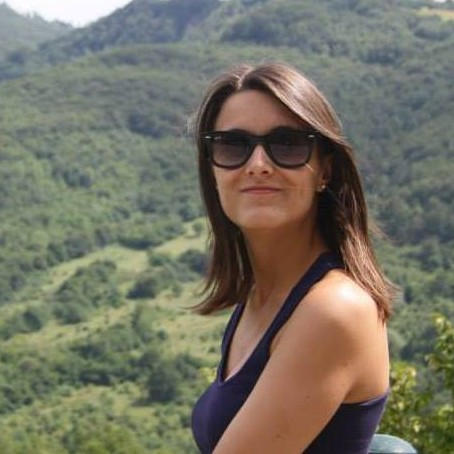
\includegraphics[width=4cm, keepaspectratio]{img/gessica_crop.jpg}
  ~
  ~
	\section{Address}
	68, Aldo Moro,
	Comunanza (AP), 63087, Italy
    ~
	\section{Tel \& Skype}
    +39 339 505 0697 \vspace{3pt}
    gessica.trivelli\\@gmail.com
    ~
	\section{Mail}
    \href{mailto:gessica.trivelli@gmail.com}{\textbf{gessica.trivelli@}\\gmail.com}
    ~
    \section{Personal Informations}
	\textbf{Nationality}: Italian
	\textbf{Birthday}: April 14
	~
\end{aside}

\section{Education}
\begin{entrylist}
	\entry
	{2016 - Now}
	{Postgraduate Specialization in Midwifery [\small EQF 7]}
	{\\Scuola Elementale di Arte Ostetrica, Florence}
	{50 ECM Specialization Course - 194 hours - on the following topic: \emph{Pelvic floor's health in female cycle: education, prevention re-education and treatment of perineal dysfunction using a midwifery-led approach.}\\}
	
	\entry
	{2014 - Now}
	{Master's Degree in Nursing and Midwifery [\small EQF 7]}
	{\\Tor Vergata, University of Rome}
	{Graduation in April 2017. \\Internship - thesis at \textit{"Istituto Superiore di Sanita'"} on the following topic: \textit{Health knowledge, attitudes and practice of midwifery students, pregnant women and midwives on umbilical cord clamping and cord blood stem cells transplantation.}\\}
	
	\entry
	{2010 - 2014}
	{Bachelor's Degree in Midwifery [\small EQF 6]}
	{\\Tor Vergata, University of Rome}
	{First class with honors.\\
	Internship in Rome in several hospitals: \textit{Policlinico Tor Vergata}, \textit{Azienza Ospedaliera San Giovanni Addolorata}, \textit{Ospedale Fatebenefratelli San Giovanni Calibita} and \textit{Policlinico Casilino}.\\
	Thesis title: \textit{Survey on Women's Positions during Labour and Delivery: Evaluation of Maternal and Foetal Outcomes.}\\}

	\entry
	{2005-2010}
	{Scientific Disploma [\small EQF 4]}
	{\\Scientific High School "A. Gentili", Sarnano (MC)}
	{}
\end{entrylist}

\section{Experience}
\begin{entrylist}
  \entry
  {2015 - Now}
  {Collaborator}
  {\\CreAttivaMente Ostetriche}
  {Co-administrator of the blog \href{http://creattivamenteostetriche2012.blogspot.it/}{CreAttivaMente Ostetriche}. 
  	Secretaryship and ECM-course co-oragnisation.\\}
  
  \entry
    {2010 - 2010}
    {Volunteer}
    {\\Croce Rossa Italiana - Italian Commitee of Sibillini}
    {\\}
\end{entrylist}

\newpage
\begin{aside}
	\section{IT Skills}
	\textbf{macOS}
\includegraphics[scale=0.40]{img/5stars.png}
	\textbf{Windows}
\includegraphics[scale=0.40]{img/5stars.png}
	\textbf{Office}
\includegraphics[scale=0.40]{img/5stars.png}
	\textbf{iWork}
\includegraphics[scale=0.40]{img/4stars.png}
	\textbf{Epi-Info}
\includegraphics[scale=0.40]{img/3stars.png}
	\textbf{Pubmed}
\includegraphics[scale=0.40]{img/5stars.png}
	~
	~
	\section{Relational Skills}
	Women-centred care,promoting information and free decision making, through skills such as \textbf{counselling}, \textbf{empathy} and \textbf{active listening}.
\end{aside}


\section{Technical Skills}
	\begin{itemize}
		\item Problem solving
		\item Use of brand new and innovative didactic models
		\item Adulthood education
		\item Planning, implementation and evaluation of clinical, organizational and pedagogical topics
		\item Quantitative and qualitative research in clinical, organizational and pedagogical fields
		\item Evaluation of care services (e.g. quality, pertinence, safety and cheapness).
	\end{itemize}
\vspace{10pt}
\section{Honours \& Awards}
\begin{entrylist}
	\entry
	{06/2016}
	{Tutoring scholaship}
	{\\Tor Vergata, University of Rome}
	{}
	{}
\end{entrylist}
\vspace{-35pt}
\section{Certifications}
\begin{entrylist}
  \entry
	  {2016}
	  {Emergencies during delivery.}
	  {\\CreAttivaMente Ostetriche, Rome}
	  {16 hours course - using medical mannequin.\\}
  \entry
	  {2015}
	  {Advanced skills to support breastfeeding.}
	  {\\CreAttivaMente Ostetriche, Rome}
	  {16 hours course.\\}
  \entry
	  {2015}
	  {Management of infertility - education, information and communication in IVF.}
	  {\\Ministero della Salute}
	  {8 hours course.\\}
  \entry
  {2014}
  {Breastfeeding: counselling practical course, OMS/UNICEF model.}
  {\\Tor Vergata, University of Rome}
  {40 hours course.\\}
\end{entrylist}
\vspace{-20pt}
\section{Languages}
\begin{table*}[!h]
	\centering
	\begin{tabular}{ p{3cm} p{3cm} p{3cm} p{3cm} }
		& \textbf{Writing} 	& \textbf{Speaking} & \textbf{Listening}			\\ 
		\textbf{Italian:}	& \multicolumn{3}{c}{Mother-tongue}					\\ 
		\textbf{English:} 	& B1 				& B1 			& B1			\\ 
		\textbf{French:}	& High School 		& High School	& High School	\\
	\end{tabular}
\end{table*}
~
\begin{flushleft}
\emph{December 6th, 2016}
\end{flushleft}
\begin{flushright}
\emph{Gessica Trivelli}
\end{flushright}

\end{document}
